\documentclass[twocolumn,a4j]{jsarticle}
\setlength{\topmargin}{-20.4cm}
\setlength{\oddsidemargin}{-10.4mm}
\setlength{\evensidemargin}{-10.4mm}
\setlength{\textwidth}{18cm}
\setlength{\textheight}{26cm}

\usepackage[top=15truemm,bottom=25truemm,left=20truemm,right=20truemm]{geometry}
\usepackage[latin1]{inputenc}
\usepackage{amsmath}
\usepackage{amsfonts}
\usepackage{amssymb}
\usepackage[dvipdfmx]{graphicx}
\usepackage[dvipdfmx]{color}
\usepackage{listings}
\usepackage{listings,jvlisting}
\usepackage{geometry}
\usepackage{framed}
\usepackage{color}
\usepackage[dvipdfmx]{hyperref}
\usepackage{ascmac}
\usepackage{enumerate}
\usepackage{tabularx}
\usepackage{cancel}
\usepackage{scalefnt}

\renewcommand{\figurename}{Fig.}
\renewcommand{\tablename}{Table }

\lstset{
basicstyle={\ttfamily},
identifierstyle={\small},
commentstyle={\smallitshape},
keywordstyle={\small\bfseries},
ndkeywordstyle={\small},
stringstyle={\small\ttfamily},
frame={tb},
breaklines=true,
columns=[l]{fullflexible},
xrightmargin=0zw,
xleftmargin=3zw,
numberstyle={\scriptsize},
stepnumber=1,
numbersep=1zw,
lineskip=-0.5ex
}

\makeatletter
\def\@maketitle
{
\begin{center}
{\LARGE \@title \par}
\end{center}
\begin{flushright}
{\large \@date}\\
{\large{京都工芸繊維大学 工芸科学科 機械工学課程}}\\
{\large \@author}
\end{flushright}
\par\vskip 1.5em
}
\makeatother

\setcounter{tocdepth}{3}

\author{来代 勝胤}
\title{令和3年度 10月度 報告書}
\date{2021/10/26}

\begin{document}
\columnseprule=0.1mm

\maketitle
\section*{報告内容}
\begin{enumerate}[1.]
    \item 校正実験結果を用いた出力値の換算
    \item 校正実験の再実施
    \item 今月の進捗と11月の予定
\end{enumerate}

\section{校正実験結果を用いた出力値の換算}
以下の手順で,校正実験結果を用いて,
実験データの出力電圧から実際の入力荷重の算出を試みた.
\begin{enumerate}[(i)]
    \item ロードセルと荷重の関係式の導出
    \item ロードセルとひずみセンサの関係式の導出
    \item ひずみセンサと入力荷重の関係式の導出
    \item 実験データの荷重への換算
\end{enumerate}
\subsection{ロードセルと荷重の関係式の導出}
2021年6月18日に実施した校正実験結果より,
ロードセルと荷重の関係式を算出した.\par
ロードセルの出力(横軸)及びロードセルの引張方向に入力した荷重(縦軸)の関係を
表した図は,以下のFig.1のようになった.
\begin{figure}[htbp]
    \footnotesize
    \begin{center}
        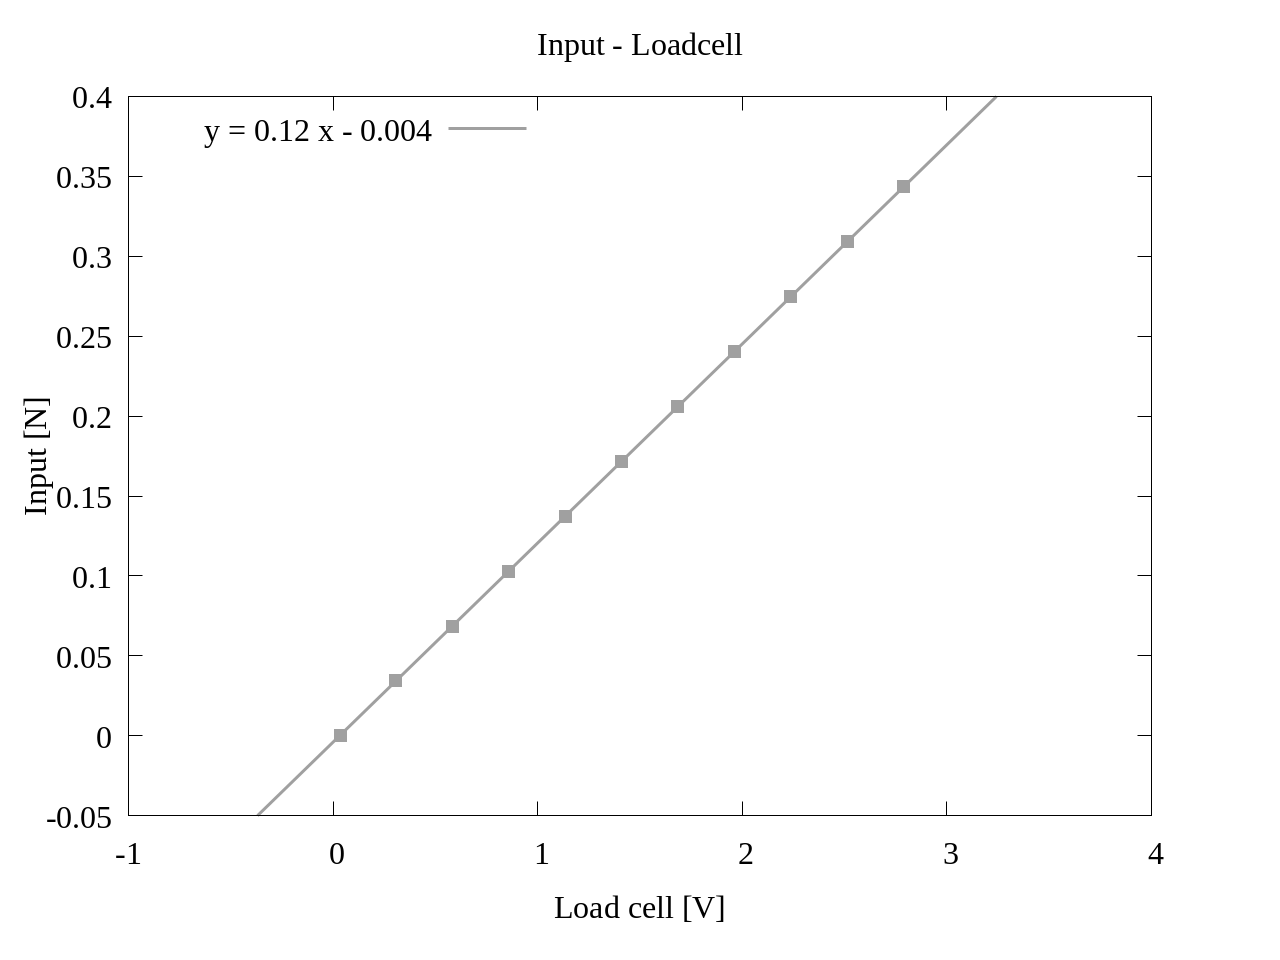
\includegraphics[width=85mm]{../images/02_force&line.png}
        \caption{Loadcell's input and output}
    \end{center}
\end{figure}

また,最小二乗法を用いて近似式を算出し,
$x$をロードセルの出力,$y$を荷重として,
以下の式(1)の結果を得ることができた.
\begin{eqnarray}
    y = 0.12 x - 0.004
\end{eqnarray}

\subsection{ロードセルとひずみセンサの関係式の導出}
2021年6月21日に実施した実験結果より,
ロードセルとひずみセンサの関係式を導出した.\\
ロードセルの出力(横軸)とタイヤモデルに取り付けられた
ひずみセンサの出力(縦軸)の関係を以下のFig.2,Fig.3に示す.
\begin{figure}[htbp]
    \footnotesize
    \begin{center}
        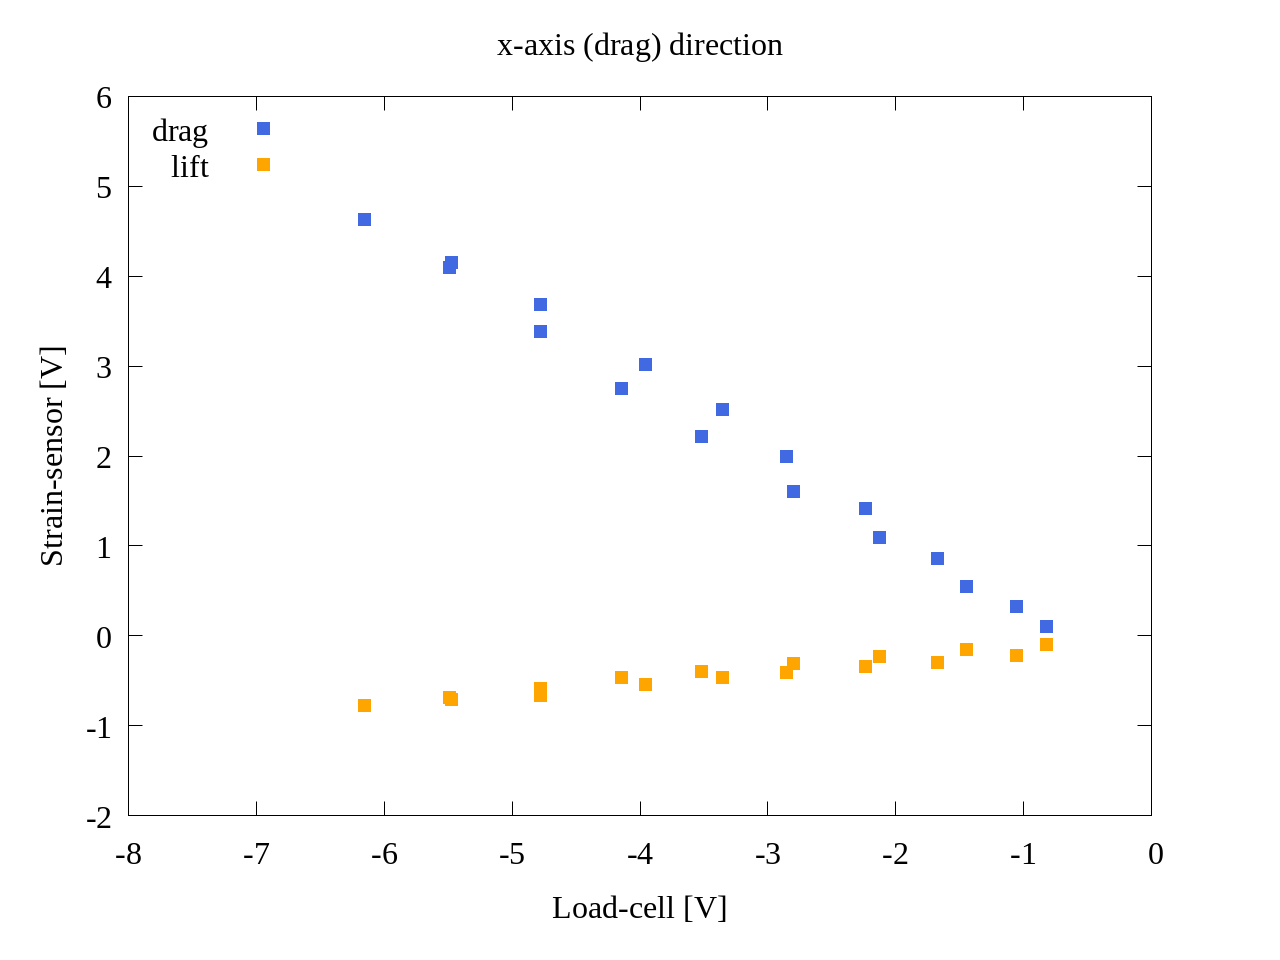
\includegraphics[width=85mm]{../images/05_strainsensor-loadcell_x.png}
        \caption{Correlation of load-cell and strain-sensors (x-axis)}
        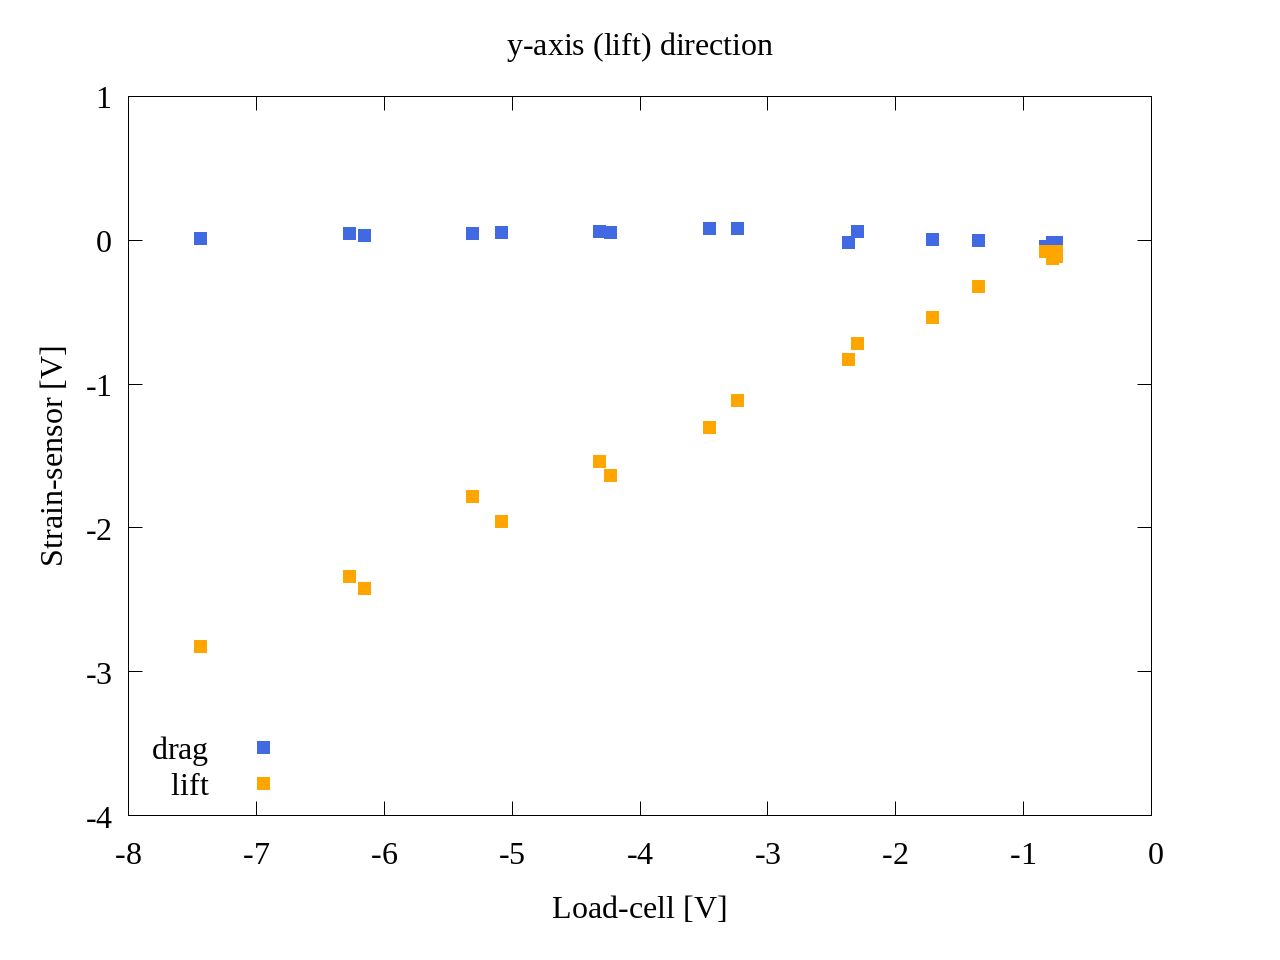
\includegraphics[width=85mm]{../images/06_strainsensor-loadcell_y.png}
        \caption{Correlation of load-cell and strain-sensors (y-axis)}
    \end{center}
\end{figure}

\newpage
\subsection{ひずみセンサと入力荷重の関係式の導出}
2つの校正実験結果から,ひずみセンサの出力電圧と
流体力による入力荷重についての関係式を導出することができる.\\
\begin{figure}[htbp]
    \footnotesize
    \begin{center}
        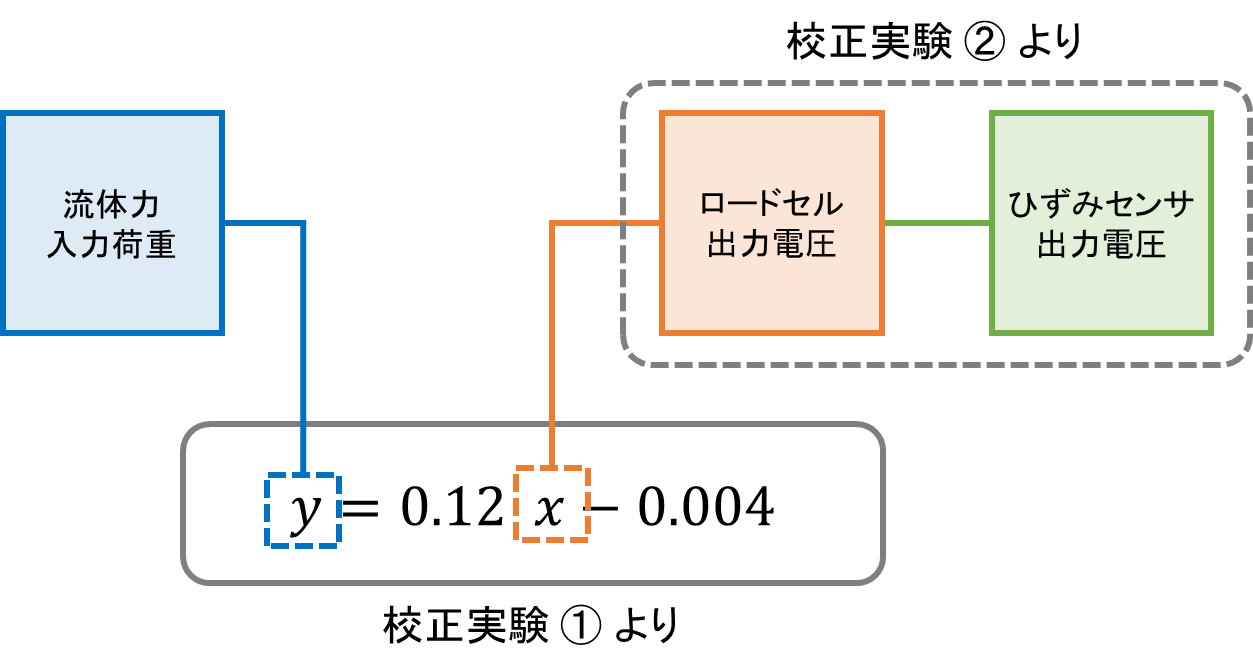
\includegraphics[width=80mm]{../images/image_03.png}
        \caption{Relationship between input and output}
    \end{center}
\end{figure}

Fig.1,Fig.2の "drag" ,Fig.3の "lift" の結果から,
ひずみセンサの出力(横軸)と入力荷重(縦軸)の関係について
以下の Fig.5に示す.\par
\begin{figure}[htbp]
    \footnotesize
    \begin{center}
        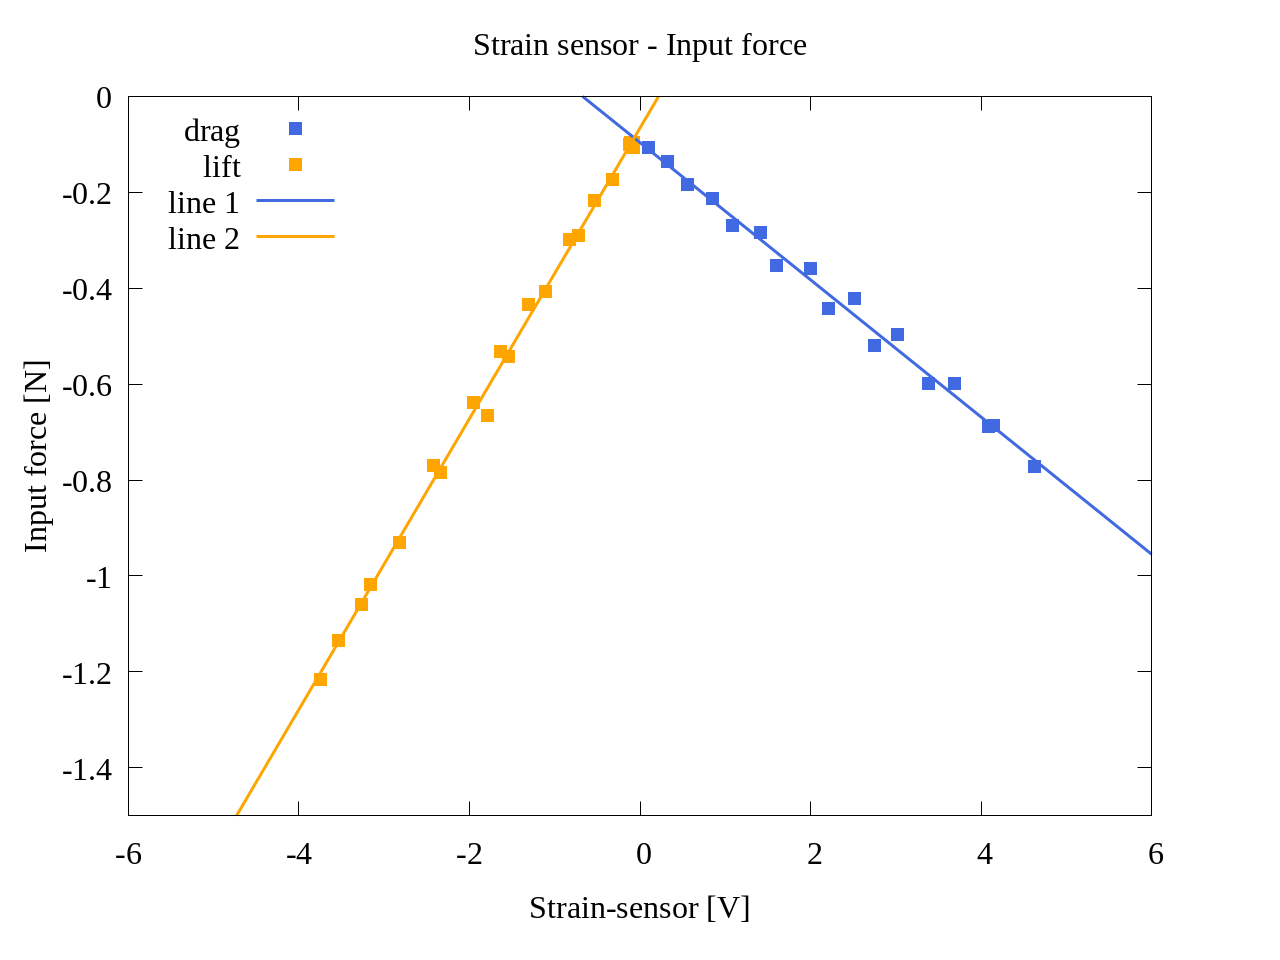
\includegraphics[width=85mm]{../images/08_strainsensor-forces&line.png}
        \caption{Correlation of input force and strain-sensors}
    \end{center}
\end{figure}
また,drag 及び lift に対して,最小二乗法を用いて近似式を算出し,
$x$をひずみセンサの出力電圧,$y$をタイヤモデルに加わる荷重として,
それぞれ以下の式(2),式(3)の近似直線を得た.
\begin{eqnarray}
    \mathrm{line 1} \; : \; y &=& -0.143 \; x - 0.10\\
    \mathrm{line 2} \; : \; y &=& 0.303 \; x - 0.07
\end{eqnarray}

\newpage
\subsection{実験データへの適用について}

ここで、導出した近似式をみると、
どちらも原点を通っていないことがわかる。
ここで、ロードセル・もしくはひずみセンサについて
原点付近で出力電圧が非線形で変化する可能性があると考えた。

また、Table.1 の実験データをみると、
校正実験で得たデータ範囲に対して、
入力荷重へと換算を適用する範囲は
非常に狭い範囲であることがわかる。

\begin{table}[htbp]
    \footnotesize
    \caption{Average of all data}
    \begin{center}
        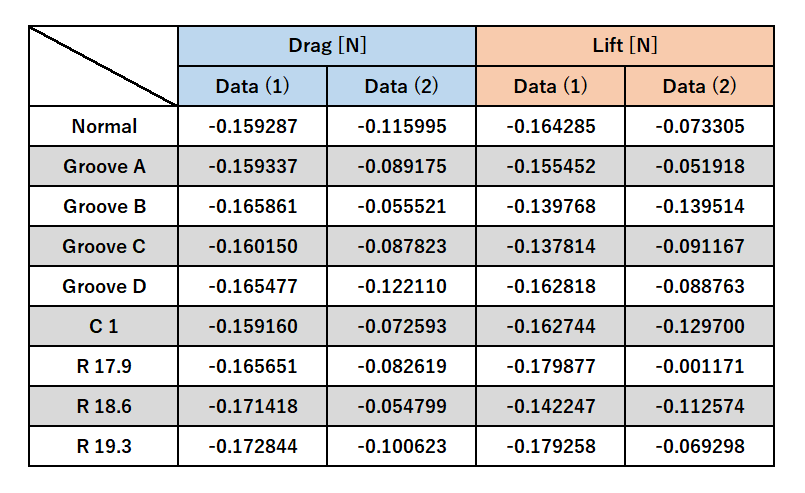
\includegraphics[width=85mm]{../images/Table_2.png}
    \end{center}
\end{table}

\begin{figure}[htbp]
    \footnotesize
    \begin{center}
        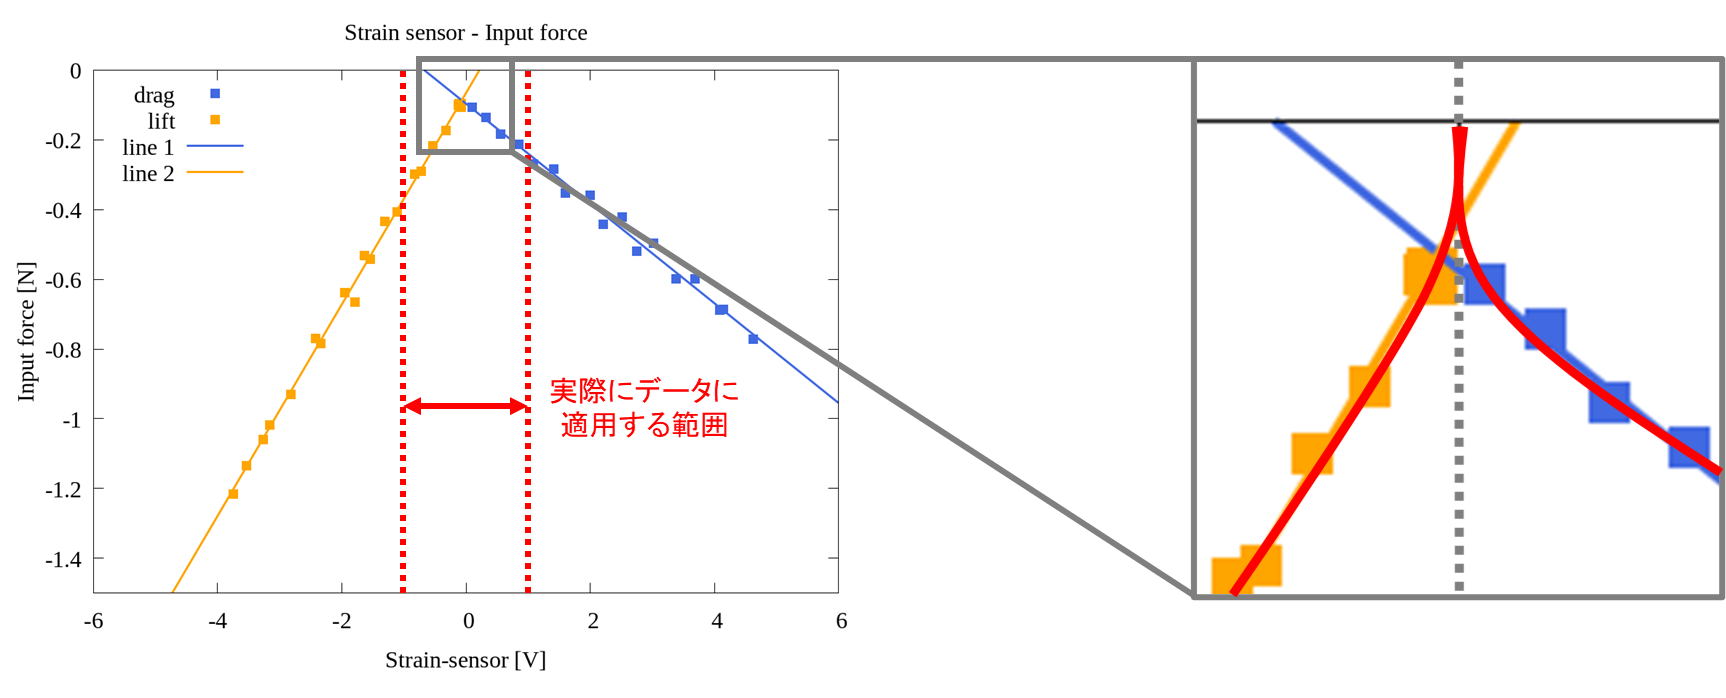
\includegraphics[width=85mm]{../images/image_04.png}
        \caption{Correlation of input force and strain-sensors}
    \end{center}
\end{figure}


\section{校正実験の再実施}
回流水槽での実験結果の換算に必要な範囲の
ロードセルとひずみゲージの関係式を得るために,
校正実験を再度実施することとした.

\subsection{校正実験装置の製作}

校正実験の再実施にあたって,実験装置Fig.7, Fig.8, Fig.9を作成した.

\begin{figure}[htbp]
    \footnotesize
    \begin{center}
        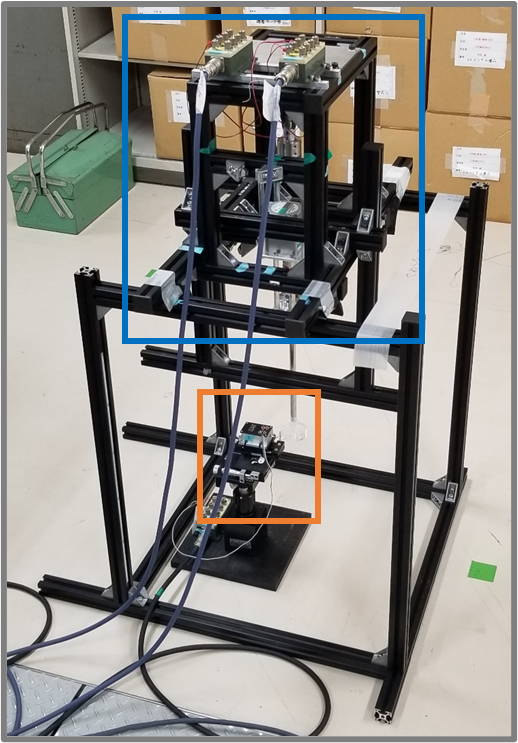
\includegraphics[width=55mm]{../images/image_05.png}
        \caption{Calibration experiment equipment}
        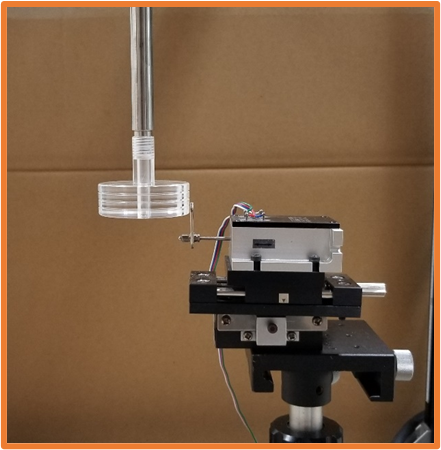
\includegraphics[width=55mm]{../images/image_06.png}
        \caption{Load cell and specimen}
        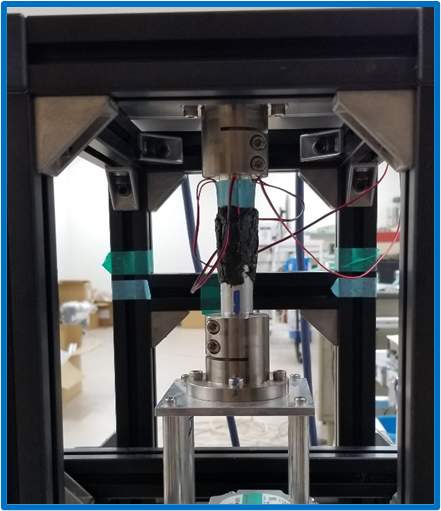
\includegraphics[width=55mm]{../images/image_07.png}
        \caption{Strain sensor}
    \end{center}
\end{figure}

\subsection{校正実験結果}

2021年10月21日(木)に,実験を行いデータを確認したが,
ストレインアンプの調整ができておらず,
正しいデータが取得できなかった.\par
したがって,早急に調整を行い実験を行う必要がある.

\section{今月の進捗と11月の予定}
\begin{itemize}
    \item [$\blacksquare$] \textgt{今月の進捗}
          \begin{itemize}
              \item [$\bullet$] ひずみセンサの出力電圧から流体力による\\
                    作用力への換算過程の確認
              \item [$\bullet$] ロードセルの出力電圧と入力荷重の関係式を得ることができた
              \item [$\bullet$] ロードセルもしくはひずみゲージの出力電圧に非線形領域が存在する可能性があることがわかった
              \item [$\bullet$] ロードセルとひずみゲージの校正実験を再度行っている\\
          \end{itemize}
    \item [$\blacksquare$] \textgt{11月の予定}
          \begin{itemize}
              \item [$\bullet$] 校正実験の再実施
              \item [$\bullet$] 実験データから出力電圧から入力荷重への換算\\
          \end{itemize}
\end{itemize}

\end{document}